\begin{frame}{Today the gender gap is \textbf{\alert{narrower}} in denser labor markets}
	\begin{columns}
		\column{0.5\textwidth}
		\begin{figure}[!h]
\centering
\caption{Gender wage gap and population density in 2020}
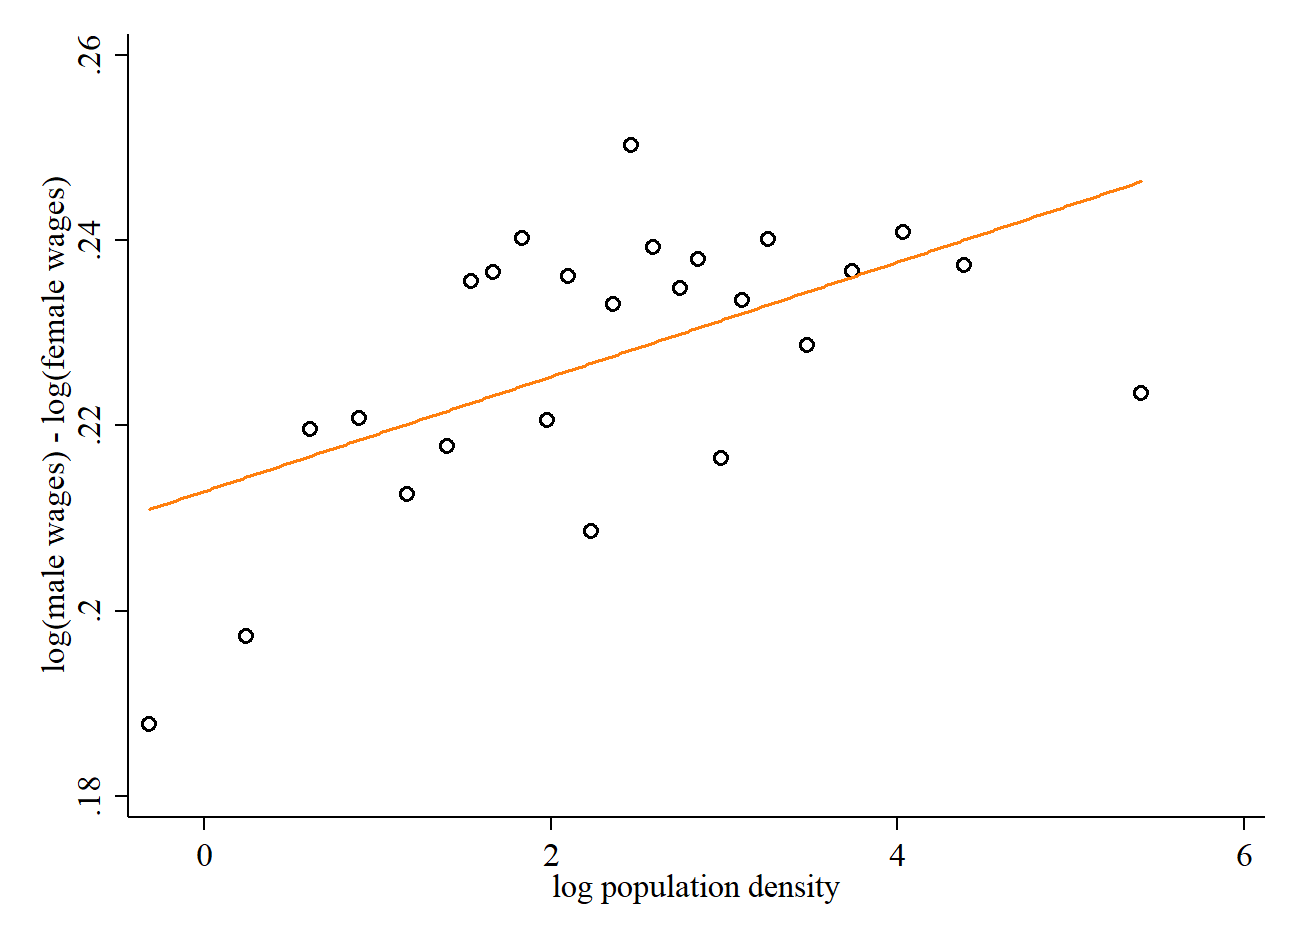
\includegraphics[width=1\textwidth]{../2_analysis/output/figures/l_czone_density_2020}
\par \begin{minipage}[h]{\textwidth}{\tiny\textbf{Note:} figure restricts to CZ with more than 1 people per km$^2$. Each point represents about 25 CZ. Year fixed effects are absorbed. Figure generated on 10 Nov 2020 at 18:18:41. Figure generated using the dofile 2\_analysis/code\_files/write\_regression\_coefplots.do.}\end{minipage}
\end{figure}

		\column{0.5\textwidth}
		The negative gradient is robust to:
		\bitem
			\item Limiting to the largest CZ 	\beamerbutton{\hyperlink{slide:map}{Largest CZ}}. 
			\item Weighting scheme 	\beamerbutton{\hyperlink{slide:map}{Weighted regression}}.
			\item Controlling for individual characteristics \beamerbutton{\hyperlink{slide:map}{Residualized wages}}.
		\eitem
	\end{columns}
\end{frame}

\begin{frame}{The negative correlation is robust}
	\begin{columns}
		\column{0.5\textwidth}
		\textbf{\alert{Limiting to the largest CZ}}
		{\tiny\begin{figure}[!h]
\centering
\caption{Gender wage gap and population density in the largest CZ}
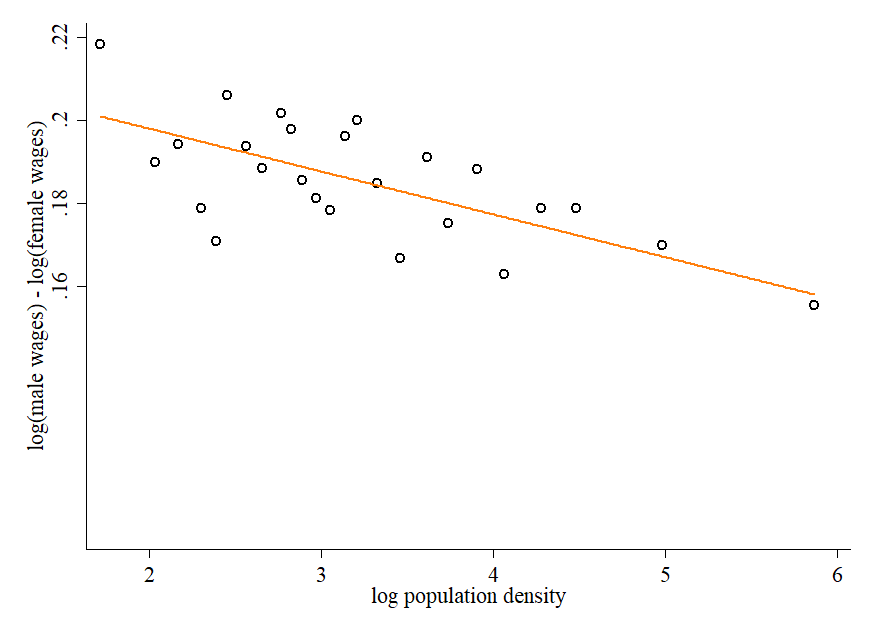
\includegraphics[width=1\textwidth]{../2_analysis/output/figures/l_czone_density_2020_big_CZ}
\par \begin{minipage}[h]{\textwidth}{\tiny\textbf{Note:} figure restricts to CZ with more than 1 people per km$^2$. Each point represents about 13 CZ. Figure generated on 23 Nov 2020 at 17:32:58. Figure generated using the dofile 2\_analysis/code\_files/write\_regression\_coefplots.do.}\end{minipage}
\end{figure}
}
		\column{0.5\textwidth}
		\textbf{\alert{Weighting by population}}
		{\tiny\begin{figure}[!h]
\centering
\caption{Gender wage gap and population density in 2020 (population weighted)}
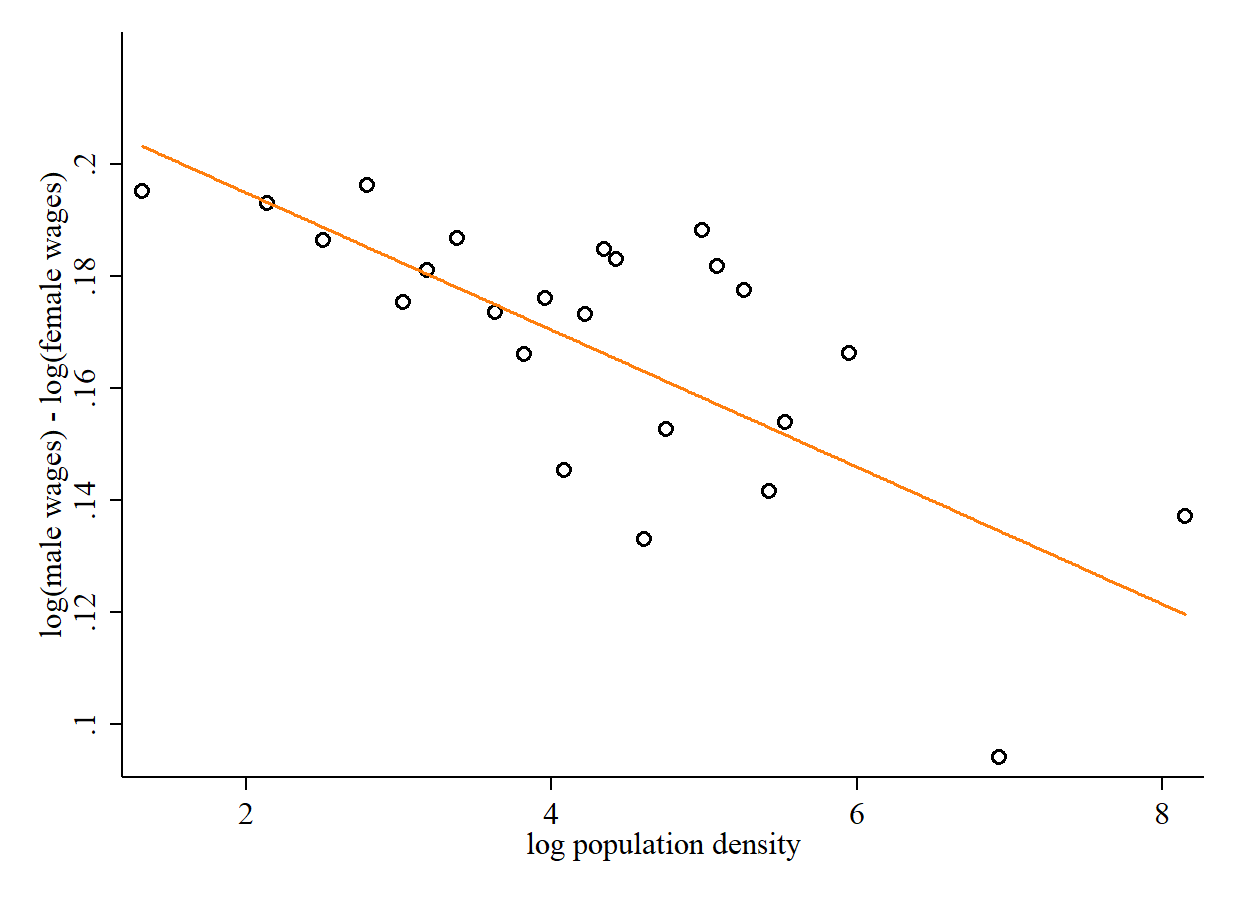
\includegraphics[width=1\textwidth]{../2_analysis/output/figures/l_czone_density_2020_w}
\par \begin{minipage}[h]{\textwidth}{\tiny\textbf{Note:} figure restricts to CZ with more than 1 people per km$^2$. Each point represents about 4 percent of the working age population. Figure generated on 17 Nov 2020 at 13:42:00. Figure generated using the dofile 2\_analysis/code\_files/write\_regression\_coefplots.do.}\end{minipage}
\end{figure}
}
	\end{columns} 
\end{frame}


\begin{frame}{It is robust to accounting for individual characteristics}
	\begin{columns}
		\column{.5\textwidth}
		\begin{figure}[!h]
\centering
\caption{Gender wage gap and population density in 2020 (population weighted)}
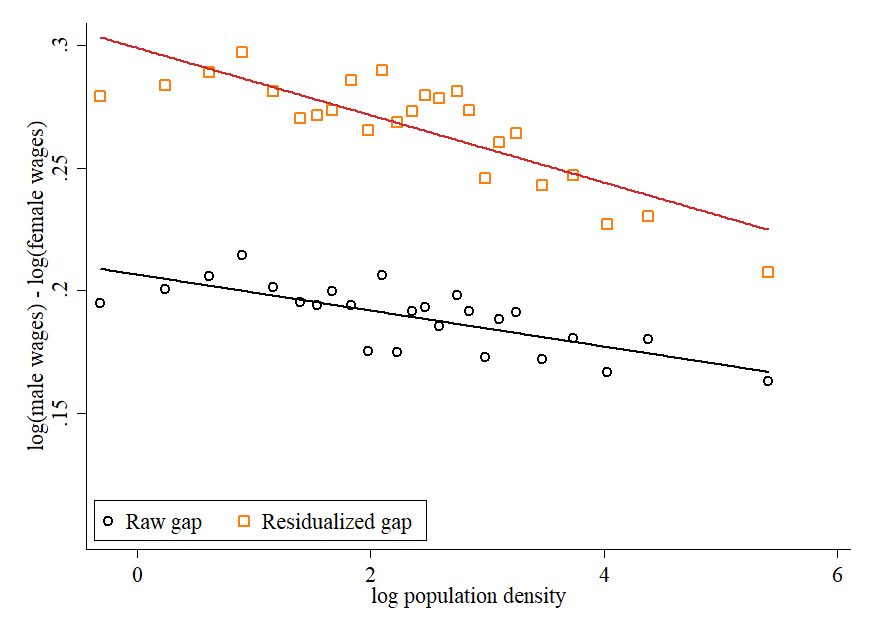
\includegraphics[width=1\textwidth]{../2_analysis/output/figures/l_czone_density_2020_hum}
\par \begin{minipage}[h]{\textwidth}{\tiny\textbf{Note:} figure restricts to CZ with more than 1 people per km$^2$. Each point represents about 4 percent of the working age population. Figure generated on 10 Nov 2020 at 18:18:43. Figure generated using the dofile 2\_analysis/code\_files/write\_regression\_coefplots.do.}\end{minipage}
\end{figure}

		\column{.5\textwidth}
	\end{columns} 
\end{frame}


\begin{frame}{The gender-gap density gradient has declined since 1970}
\begin{columns}
	\column{0.5\textwidth}
	\begin{figure}[!h]
\centering
\caption{Gender wage gap and population density}
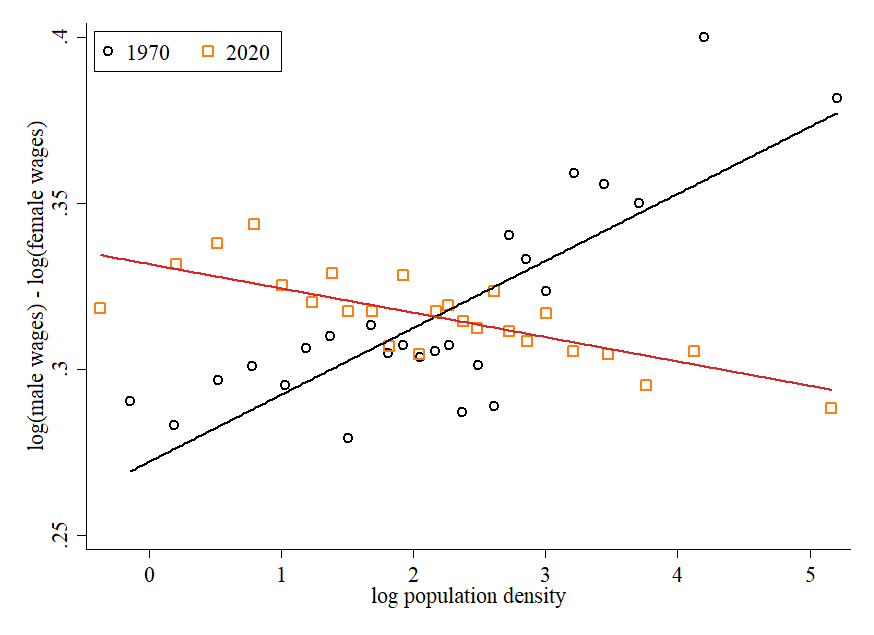
\includegraphics[width=1\textwidth]{../2_analysis/output/figures/l_czone_density_1970_vs_2020}
\par \begin{minipage}[h]{\textwidth}{\tiny\textbf{Note:} figure restricts to CZ with more than 1 people per km$^2$. Each point represents about 25 CZ. Year fixed effects are absorbed. Figure generated on 17 Nov 2020 at 13:42:02. Figure generated using the dofile 2\_analysis/code\_files/write\_regression\_coefplots.do.}\end{minipage}
\end{figure}

	\beamerbutton{\hyperlink{slide:map}{Graph without absorb}} 
	\column{0.5\textwidth}
	\begin{figure}[!h]
\centering
\caption{Coefficient on population density $ \beta_t $}
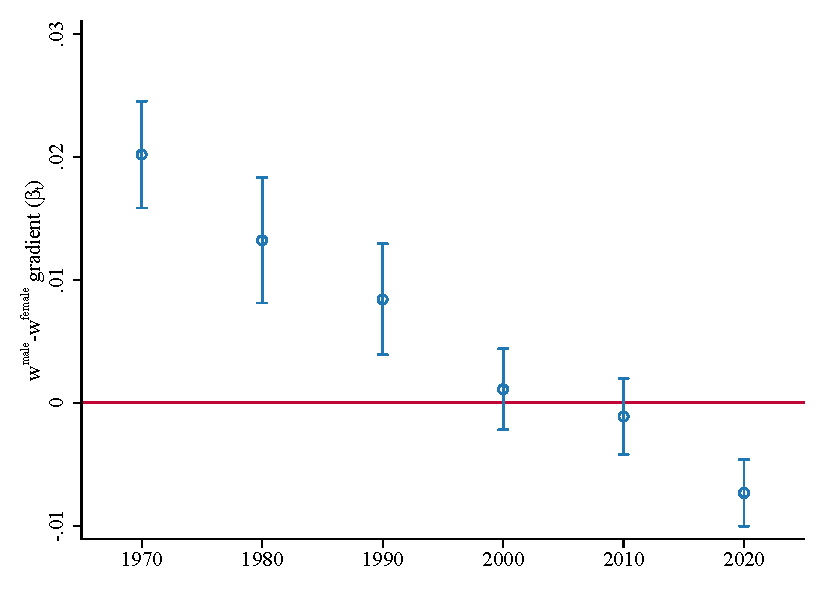
\includegraphics[width=1\textwidth]{../2_analysis/output/figures/baseline_l_czone_density_full_time}
\par \begin{minipage}[h]{\textwidth}{\tiny\textbf{Note:} figure restricts to CZ with more than 1 people per km$^2$. Bars show 95\% confidence intervals. Standard errors clustered at the CZ level. Figure generated on 11 Nov 2020 at 19:32:51. Figure generated using the dofile 2\_analysis/code\_files/write\_regression\_coefplots.do.}\end{minipage}
\end{figure}

	\beamerbutton{\hyperlink{slide:map}{With individual controls}}
\end{columns}
\end{frame}

\begin{frame}{Robustness}
	The change in the gradient is robust to:
	\bitem 
		\item Limiting regressions to the biggest CZ	\beamerbutton{\hyperlink{slide:map}{biggest CZ}}.
		\item Using weighting schemes commonly used in the literature (estimates become much more imprecise) \beamerbutton{\hyperlink{slide:map}{population weighting}}
		\item Using only within-region / within-state variation  \beamerbutton{\hyperlink{slide:map}{adding FE}}
		\item Adjusting wages by: age, education, foreign born dummy, and education \beamerbutton{\hyperlink{slide:map}{residualizing wages}}.
		\item Using log of CZ population as independent variable \beamerbutton{\hyperlink{slide:map}{population as density measure}}.
	\eitem 
\end{frame}


\begin{frame}{Robustness}
	\begin{columns}
		\column{0.5\textwidth}
		\begin{figure}[!h]
\centering
\caption{Coefficient on population density $ \beta_t $ for largest CZ}
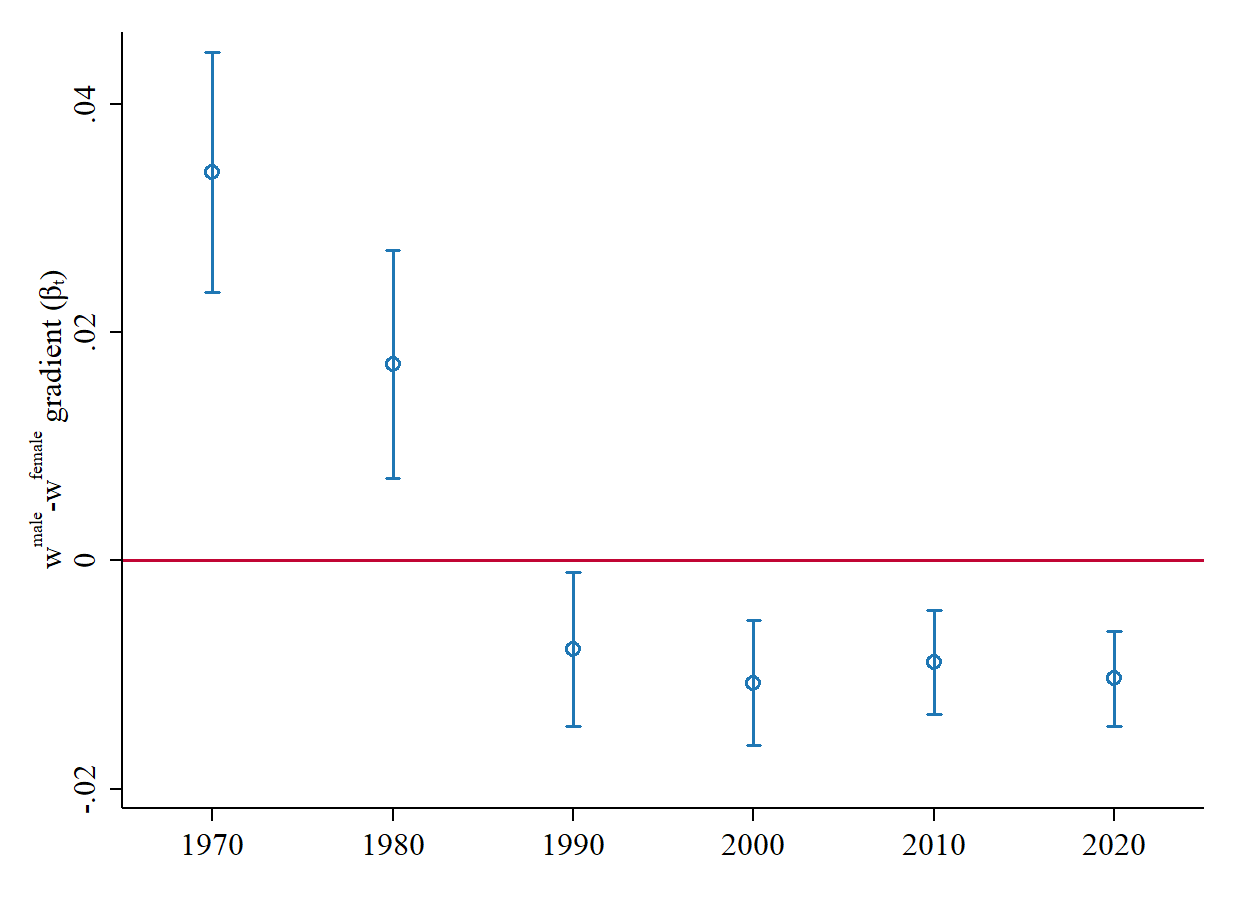
\includegraphics[width=1\textwidth]{../2_analysis/output/figures/baseline_large_l_czone_density_full_time}
\par \begin{minipage}[h]{\textwidth}{\tiny\textbf{Note:} figure restricts to more than 2 people per km$^2$ in 1950. Bars show 95\% confidence intervals. Standard errors clustered at the CZ level. Figure generated on 11 Nov 2020 at 19:32:52. Figure generated using the dofile 2\_analysis/code\_files/write\_regression\_coefplots.do.}\end{minipage}
\end{figure}

		\beamerbutton{\hyperlink{slide:map}{With individual controls}}
		\column{0.5\textwidth}
		\begin{figure}[!h]
\centering
\caption{Coefficient on population density $ \beta_t $ (population weighted)}
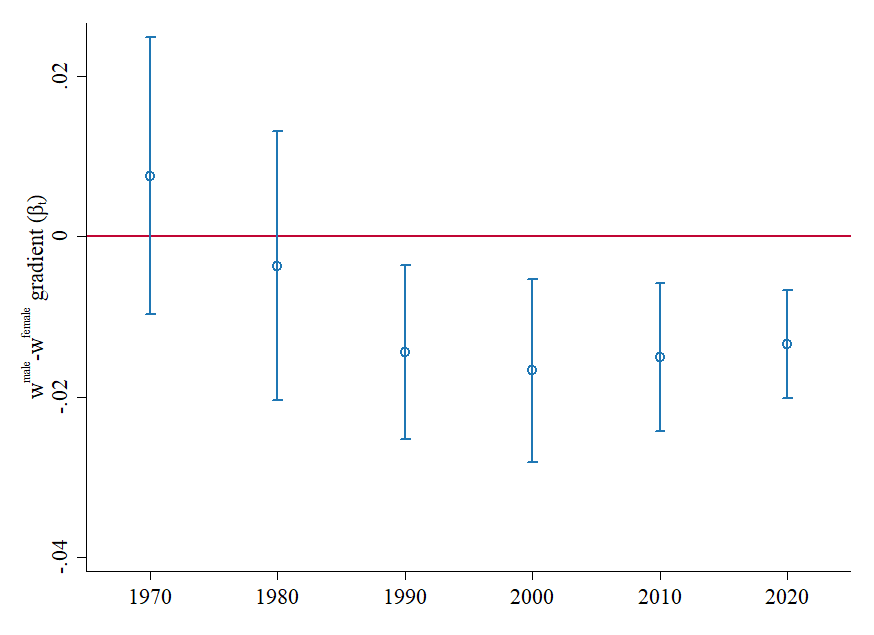
\includegraphics[width=1\textwidth]{../2_analysis/output/figures/baseline_w_l_czone_density_full_time}
\par \begin{minipage}[h]{\textwidth}{\tiny\textbf{Note:} figure restricts to more than 1 people per km$^2$ in 1950. Regressions weighted by the CZ population in 1970. Bars show 95\% confidence intervals. Standard errors clustered at the CZ level. Figure generated on 17 Nov 2020 at 13:42:03. Figure generated using the dofile 2\_analysis/code\_files/write\_regression\_coefplots.do.}\end{minipage}
\end{figure}

		\beamerbutton{\hyperlink{slide:map}{Graph without absorb}} 
	\end{columns}
\end{frame}

\begin{frame}{Robustness}
	\begin{columns}
		\column{0.5\textwidth}
		\begin{figure}[!h]
\centering
\caption{Coefficient on population density $ \beta_t $ adding fixed effects}
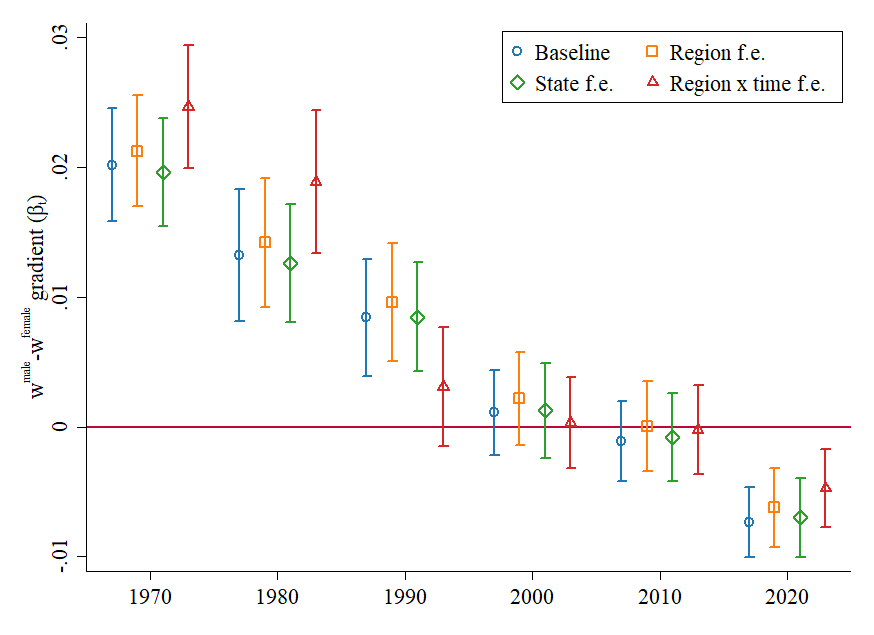
\includegraphics[width=1\textwidth]{../2_analysis/output/figures/baseline_fe_l_czone_density_full_time}
\par \begin{minipage}[h]{\textwidth}{\tiny\textbf{Note:} figure restricts to more than 1 people per km$^2$ in 1950. Bars show 95\% confidence intervals. Standard errors clustered at the CZ level. Figure generated on 17 Nov 2020 at 13:42:05. Figure generated using the dofile 2\_analysis/code\_files/write\_regression\_coefplots.do.}\end{minipage}
\end{figure}

		\beamerbutton{\hyperlink{slide:map}{With individual controls}}
		\column{0.5\textwidth}
	    { \tiny	\begin{figure}[!h]
\centering
\caption{Coefficient on population density $ \beta_t $ controlling for worker characteristics}
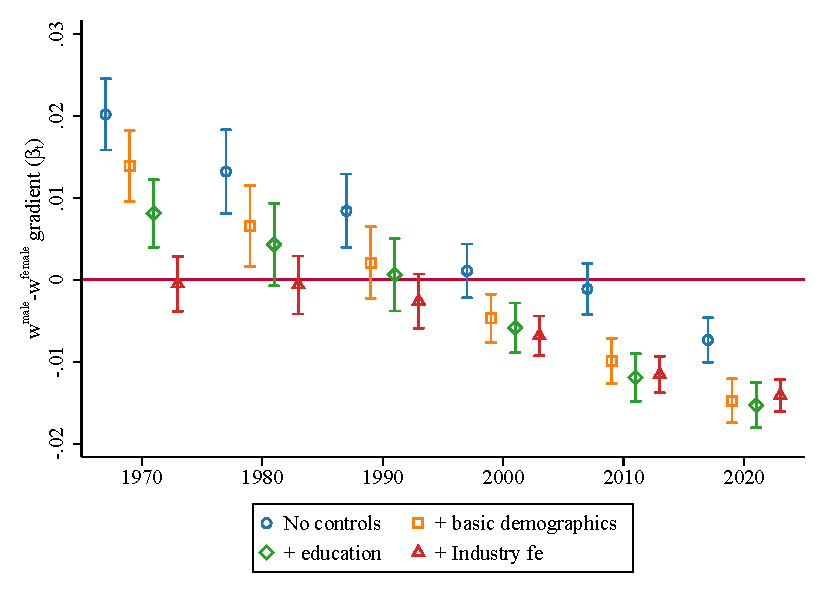
\includegraphics[width=.6\textwidth]{../2_analysis/output/figures/with_control_gradients_individual_l_czone_density_full_time}
\par \begin{minipage}[h]{\textwidth}{\tiny\textbf{Note:} figure restricts to CZ with more than 1 people per km$^2$. The regressions are done on data aggregated at the CZ level after residualizing individual-level characteristics. Bars show 95\% confidence intervals. Errors clustered at the CZ-level.}\end{minipage}
\end{figure}
}
		\beamerbutton{\hyperlink{slide:map}{Graph without absorb}} 
	\end{columns}
\end{frame}

\begin{frame}{The gradient decline in perspective: several benchmarks}
	\bitem
		\item Translate coefficients in terms of gap from small vs densest CZ
		\item Coefficients are percent of gender gap sd.
		\item Change in coefficients in terms of urban wage premium.
	\eitem 
\end{frame}


\begin{frame}{A tale of women's success and male decline in denser labor markets}
	\begin{columns}
		\column{0.5\textwidth}
		\begin{figure}[!h]
\centering
\caption{Coefficient on population density $ \beta_t $}
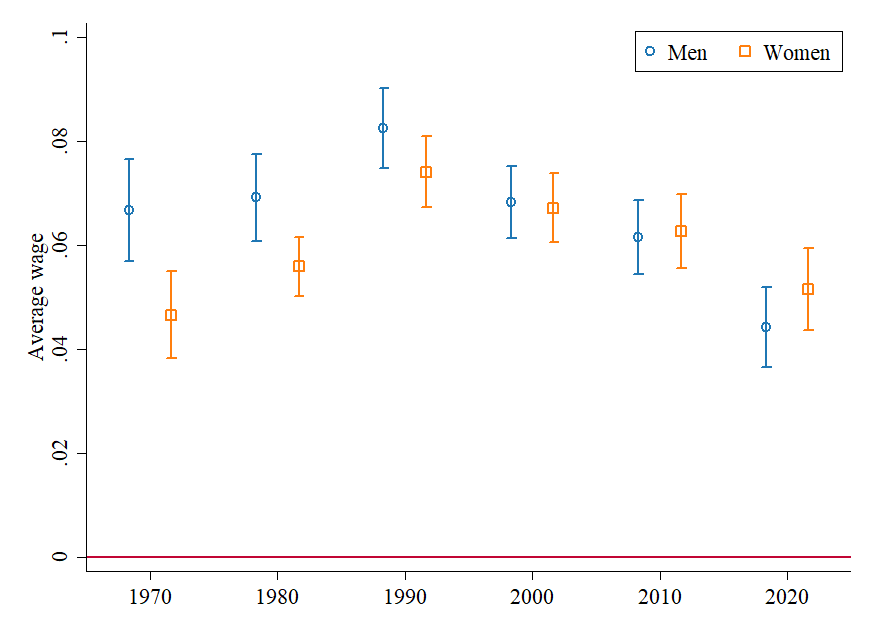
\includegraphics[width=1\textwidth]{../2_analysis/output/figures/premium_by_gender_full_time}
\par \begin{minipage}[h]{\textwidth}{\tiny\textbf{Note:} figure restricts to CZ with more than 1 people per km$^2$. Bars show 95\% confidence intervals. Standard errors clustered at the CZ level. Figure generated on  8 Nov 2020 at 14:00:12. Figure generated using the dofile 2\_analysis/code\_files/write\_regression\_coefplots.do.}\end{minipage}
\end{figure}

		\beamerbutton{\hyperlink{slide:map}{Graph without absorb}}
		\column{0.5\textwidth}
		\begin{figure}[!h]
\centering
\caption{Coefficient on population density $ \beta_t $}
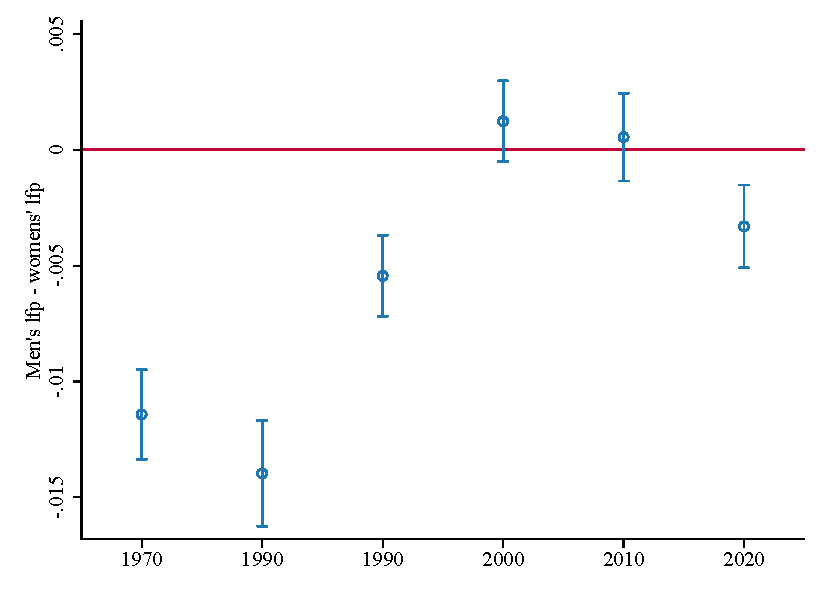
\includegraphics[width=1\textwidth]{../2_analysis/output/figures/lfp_gap_full_time}
\par \begin{minipage}[h]{\textwidth}{\tiny\textbf{Note:} figure restricts to CZ with more than 1 people per km$^2$. Bars show 95\% confidence intervals. Standard errors clustered at the CZ level. Figure generated on  8 Nov 2020 at 14:00:13. Figure generated using the dofile 2\_analysis/code\_files/write\_regression\_coefplots.do.}\end{minipage}
\end{figure}

		\beamerbutton{\hyperlink{slide:map}{Weighted regressions}}
		\beamerbutton{\hyperlink{slide:map}{With individual controls}}
	\end{columns}
\end{frame}



\begin{frame}{A tale of women's success and male decline in denser labor markets}
	\begin{columns}
		\column{0.5\textwidth}
		\begin{figure}[!h]
\centering
\caption{Coefficient on population density $ \beta_t $}
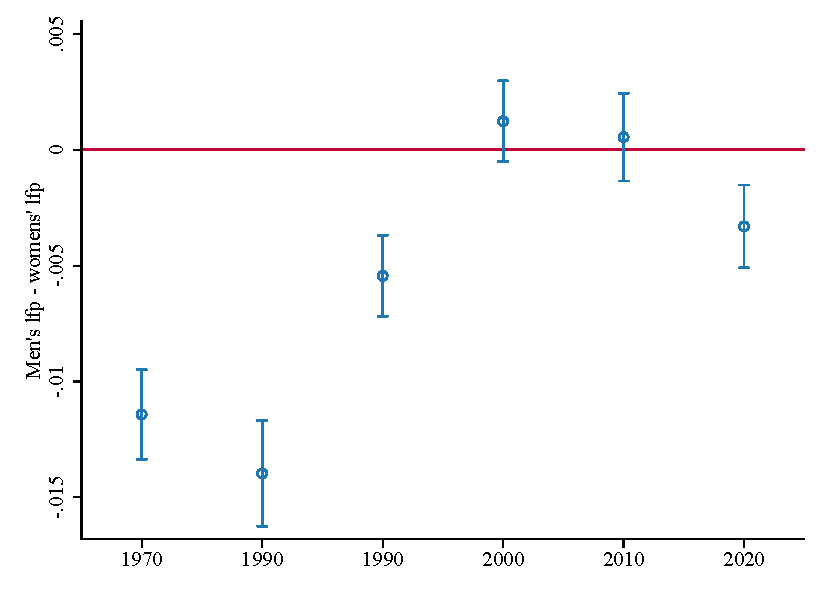
\includegraphics[width=1\textwidth]{../2_analysis/output/figures/lfp_gap_full_time}
\par \begin{minipage}[h]{\textwidth}{\tiny\textbf{Note:} figure restricts to CZ with more than 1 people per km$^2$. Bars show 95\% confidence intervals. Standard errors clustered at the CZ level. Figure generated on  8 Nov 2020 at 13:34:16. Figure generated using the dofile 2\_analysis/code\_files/write\_regression\_coefplots.do.}\end{minipage}
\end{figure}

		\beamerbutton{\hyperlink{slide:map}{Graph without absorb}}
		\column{0.5\textwidth}
		\begin{figure}[!h]
\centering
\caption{Coefficient on population density $ \beta_t $}
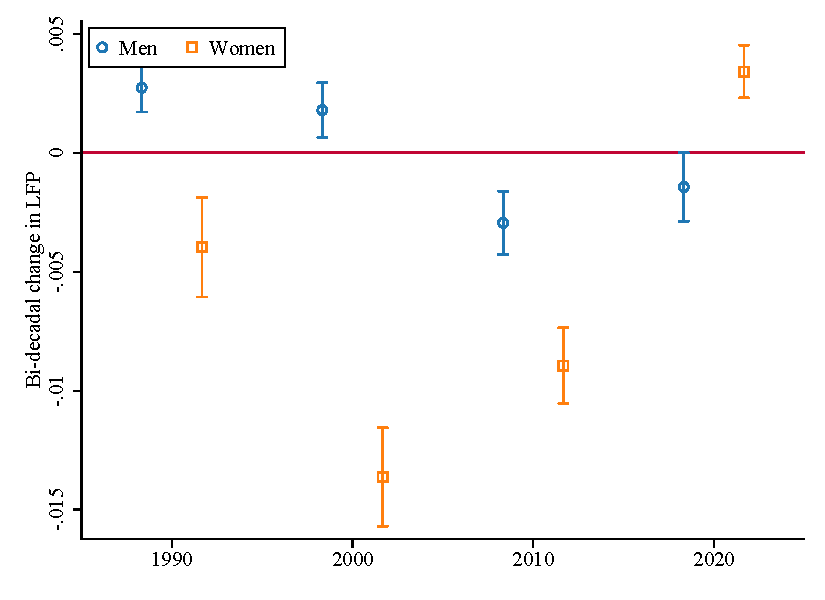
\includegraphics[width=1\textwidth]{../2_analysis/output/figures/d_lfp_gender_full_time}
\par \begin{minipage}[h]{\textwidth}{\tiny\textbf{Note:} figure restricts to CZ with more than 1 people per km$^2$. Bars show 95\% confidence intervals. Standard errors clustered at the CZ level. Figure generated on  8 Nov 2020 at 14:00:13. Figure generated using the dofile 2\_analysis/code\_files/write\_regression\_coefplots.do.}\end{minipage}
\end{figure}

		\beamerbutton{\hyperlink{slide:map}{Weighted regressions}}
		\beamerbutton{\hyperlink{slide:map}{With individual controls}}
	\end{columns}
\end{frame}


\begin{frame}{What can explain the decline in the gradient?}
	\bitem 
		\item Increased sorting of high-skill women in the densest CZ.
		\item Rise of women college education
		\item CZ industrial structure.
	\eitem 
\end{frame}
\begin{frame}{Industrial structure}
	\bitem 
	\item Increased sorting of high-skill women in the densest CZ.
	\item Rise of women college education
	\item CZ industrial structure.
	\eitem 
\end{frame}

\begin{frame}{Not readily explained by sorting on human-capital variables}
 	\begin{columns}
 		\column{0.5\textwidth}
 		\bitem
	 		\item If high-skill women increasingly sort into into denser labor markets (relative to men)$\implies$gender gaps in denser CZ will decrease faster over time.
	 		\bitem
	 		\item Decrease in the gradient should disappear once education is taken into account.
	 		\item Not supported by the data.
	 		\eitem 
 		\eitem 
		\column{0.5\textwidth}	
		 { \tiny	\begin{figure}[!h]
\centering
\caption{Coefficient on population density $ \beta_t $ controlling for worker characteristics}
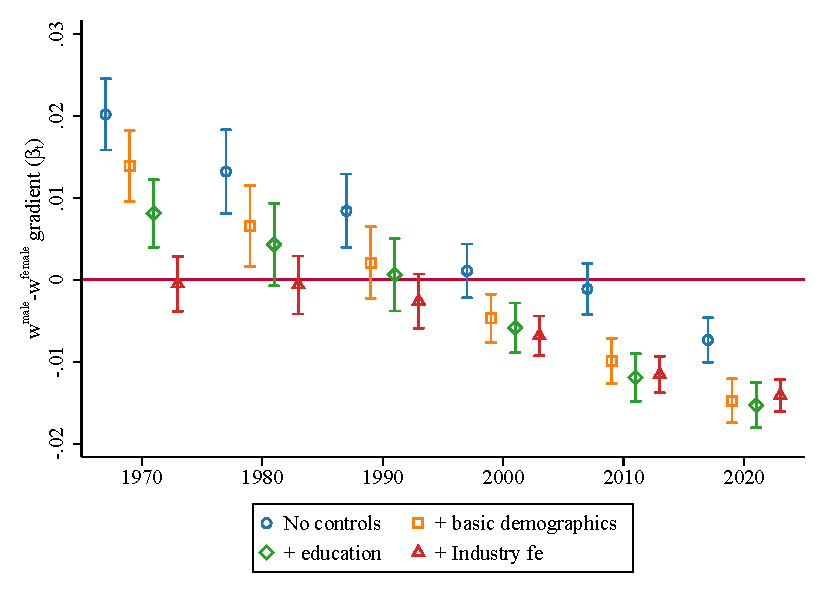
\includegraphics[width=.6\textwidth]{../2_analysis/output/figures/with_control_gradients_individual_l_czone_density_full_time}
\par \begin{minipage}[h]{\textwidth}{\tiny\textbf{Note:} figure restricts to CZ with more than 1 people per km$^2$. The regressions are done on data aggregated at the CZ level after residualizing individual-level characteristics. Bars show 95\% confidence intervals. Errors clustered at the CZ-level.}\end{minipage}
\end{figure}
}
 	\end{columns}
\end{frame}
\begin{frame}{Change in the gender gap gradient is concentrated in workers without a college degree}
	\begin{columns}
		\column{0.5\textwidth}
		\column{0.5\textwidth}
	\end{columns} 
\end{frame}

\begin{frame}{The role of industries}
	\begin{columns}
	\column{0.5\textwidth}
	\bitem
		\item My main takeaway: changes between 1970-1980 accounted by industry f.e. $\implies$ women were more able to enter into high paying occupations in denser labor markets.
	\eitem
	\column{0.5\textwidth}	
	{ \tiny	\begin{figure}[!h]
\centering
\caption{Coefficient on population density $ \beta_t $ controlling for worker characteristics}
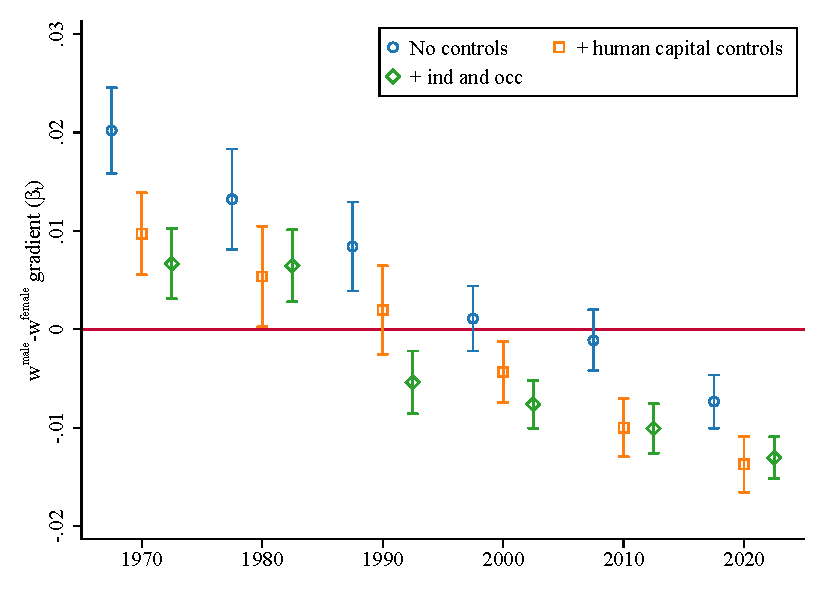
\includegraphics[width=1\textwidth]{../2_analysis/output/figures/with_ind_gradients_individual_l_czone_density_full_time}
\par \begin{minipage}[h]{\textwidth}{\tiny\textbf{Note:} figure restricts to CZ with more than 1 people per km$^2$. The regressions are done on data aggregated at the CZ level. Bars show 95\% robust confidence intervals. Standard errors clustered at the CZ level. Figure generated on 11 Nov 2020 at 19:32:54. Figure generated using the dofile 2\_analysis/code\_files/write\_regression\_coefplots.do.}\end{minipage}
\end{figure}
}
\end{columns}
\end{frame}
\begin{frame}{Is it polarization of the occupational structure?}
	\bitem
	\item 
	\eitem 
\end{frame}
\begin{frame}{Not explained by increase in inequality}
	\bitem
	\item 
	\eitem 
\end{frame}


\begin{frame}{\textbf{Fact 1:} there are persistent differences in \underline{the level} of the gender gap across CZ} 
\label{slide:fact1}
{\scriptsize\begin{center}
\begin{threeparttable}[!h]
\caption{CZ-level gender gap statistics}
\begin{tabular}{lcccccc}
\toprule
\toprule
& \multicolumn{6}{c}{\textbf{Census year}} \\
\cline{2-7}
\textbf{Statistic}&\multicolumn{1}{c}{\textbf{1970}}&\multicolumn{1}{c}{\textbf{1980}}&\multicolumn{1}{c}{\textbf{1990}}&\multicolumn{1}{c}{\textbf{2000}}&\multicolumn{1}{c}{\textbf{2010}}&\multicolumn{1}{c}{\textbf{2020}} \\
\midrule
Average gap         &        0.44         &        0.41         &        0.33         &        0.26         &        0.21         &        0.19         \\
Standard deviation  &        0.07         &        0.08         &        0.06         &        0.05         &        0.05         &        0.05         \\
\midrule\textbf{Distribution} \\
\midrule\hspace{0mm}p90&        0.53         &        0.51         &        0.40         &        0.32         &        0.26         &        0.25         \\
\hspace{0mm}p75     &        0.49         &        0.47         &        0.37         &        0.29         &        0.24         &        0.22         \\
\hspace{0mm}Median  &        0.44         &        0.41         &        0.33         &        0.26         &        0.21         &        0.19         \\
\hspace{0mm}p25     &        0.40         &        0.36         &        0.29         &        0.23         &        0.17         &        0.16         \\
\hspace{0mm}p10     &        0.35         &        0.32         &        0.26         &        0.20         &        0.15         &        0.13         \\
\bottomrule
\bottomrule
\end{tabular}
\end{threeparttable}
\end{center}
}
\textbf{\alert{Persistence:}} 20-year auto-correlation coefficient $>$ 50\%.

\beamerbutton{\hyperlink{slide:map}{Geographical pattern}}\hspace{1cm} 
\end{frame}

\begin{frame}{Fact 2: there is wide variation in the \underline{change} of gender wage gap across CZ}

\end{frame}
\begin{frame}{Fact 3: decline of the gender gap was faster in denser CZ}  				
	\begin{figure}[!h]
\centering
\caption{Change in male wage advantage in US CZ}
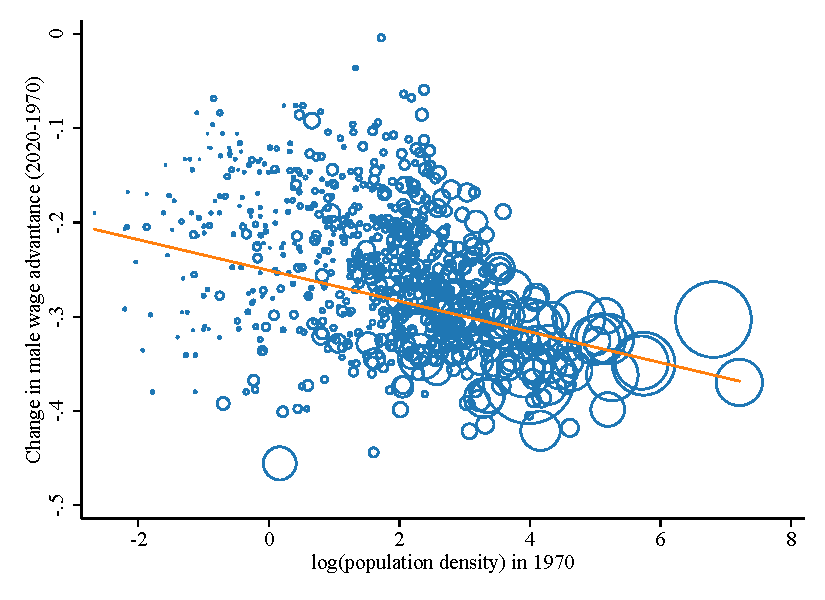
\includegraphics[width=.75\textwidth]{../2_analysis/output/figures/change_in_gap}
\end{figure}

\end{frame}
\begin{frame}{Fact 4: the gender gap - density gradient has \underline{inverted}}
	\label{slide:baseline}
	\textbf{\alert{Regression specification:}}	$w^{men}_{rt}-w^{women}_{rt}=\alpha_{rt}+\beta_{t}\ln(density)_{rt}+ \dots$
	\begin{figure}[!h]
\centering
\caption{Coefficient on population density $ \beta_t $}
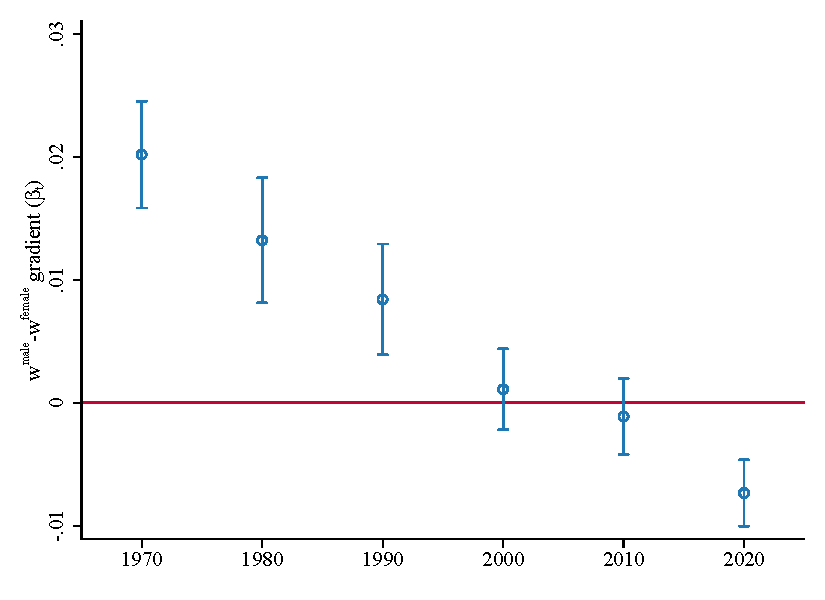
\includegraphics[width=.6\textwidth]{../2_analysis/output/figures/baseline_gradients_l_czone_density_full_time}
\par \begin{minipage}[h]{\textwidth}{\scriptsize\textbf{Note:} figure restricts to CZ with more than 1 people per km$^2$. Bars show 95\% robust confidence intervals.}\end{minipage}
\end{figure}

\end{frame}
\begin{frame}{The change in the gender-gap gradient is big}
	\bitem
		\item 
		\item Men vs women urban wage premium
	\eitem
\end{frame}
\begin{frame}{}
This change in the gradient:
\bitem
	\item is not driven \textbf{\alert{permanent}} regional differences across the US [graph adding the fixed effects].
	\item is not driven any single CZ [1970 vs 2020 graph].
	\item is not present when looking at race \beamerbutton{\hyperlink{slide:race}{race graphs}}.
	\item is also present when I zoom in on the 240 most dense labor markets [limit to the 40\% most dense labor markets]
	\item also appears when including part-time workers in the sample
\eitem	
\beamerbutton{\hyperlink{slide:interpretation}{On coefficient size}} \hspace{.5cm} 	\beamerbutton{\hyperlink{slide:distribution}{Distribution illustration}}	 \hspace{.5cm} 	\hspace{.5cm}	\beamerbutton{\hyperlink{slide:married}{Within-group graphs}}	
\end{frame}

\begin{frame}{What is driving these pattern? A mix of women's progress and men decline}
	There are two distinct periods:
	\bitem
		\item \textbf{\alert{1970-1990}:} both sexes gain in denser CZ, but women's gains are larger.
		\item \textbf{\alert{1990-2010}:} changes in the gradient are driven by men's decline in denser labor markets.
	\eitem
	
\end{frame}

\begin{frame}{How big are these coefficients?}  
		\begin{center}
\begin{threeparttable}[!h]
\caption{Male advantange changes implied by estimated elasticities}
\label{tab:IC}
\begin{tabular}{lcccccc}
\toprule
\toprule
\textbf{}&\multicolumn{1}{c}{\textbf{1970}}&\multicolumn{1}{c}{\textbf{1980}}&\multicolumn{1}{c}{\textbf{1990}}&\multicolumn{1}{c}{\textbf{2000}}&\multicolumn{1}{c}{\textbf{2010}}&\multicolumn{1}{c}{\textbf{2020}} \\
\midrule
Density elasticity $ (\beta ) $&       0.020         &       0.013         &       0.008         &       0.001         &      -0.001         &      -0.007         \\
 \hspace{3mm} s.d. wage gap &       0.073         &       0.077         &       0.060         &       0.049         &       0.049         &       0.050         \\
$ \hspace{3mm}\beta / sd $&       0.278         &       0.173         &       0.141         &       0.022         &      -0.023         &      -0.146         \\
\midrule IC range   &       0.029         &       0.019         &       0.013         &       0.002         &      -0.002         &      -0.012         \\
\hspace{3mm} (\% mean gap) &       0.065         &       0.047         &       0.040         &       0.007         &      -0.009         &      -0.064         \\
 \midrule 90 - 10 pctile range  &       0.061         &       0.040         &       0.027         &       0.004         &      -0.004         &      -0.025         \\
\hspace{3mm} (\% mean gap)&       0.137         &       0.097         &       0.082         &       0.014         &      -0.018         &      -0.133         \\
\bottomrule
\bottomrule
\end{tabular}
\begin{tablenotes}
\item \footnotesize \textit{Note:} changes based on unweighted estimated elasticities. Sample restricted to full-time year-round workers. Table generated on 28 Sep 2020 at 15:15:18.
\end{tablenotes}
\end{threeparttable}
\end{center}

\end{frame}

\begin{frame}{What can account for the change in the density-gradient?}
	\label{slide:controls}
	\textbf{\alert{Regression specification:}} $w^{men}_{rt}-w^{women}_{rt}=\alpha_{rt}+\beta_{t}\ln(density)_t$
	\begin{figure}[!h]
\centering
\caption{Coefficient on population density $ \beta_t $ controlling for worker characteristics}
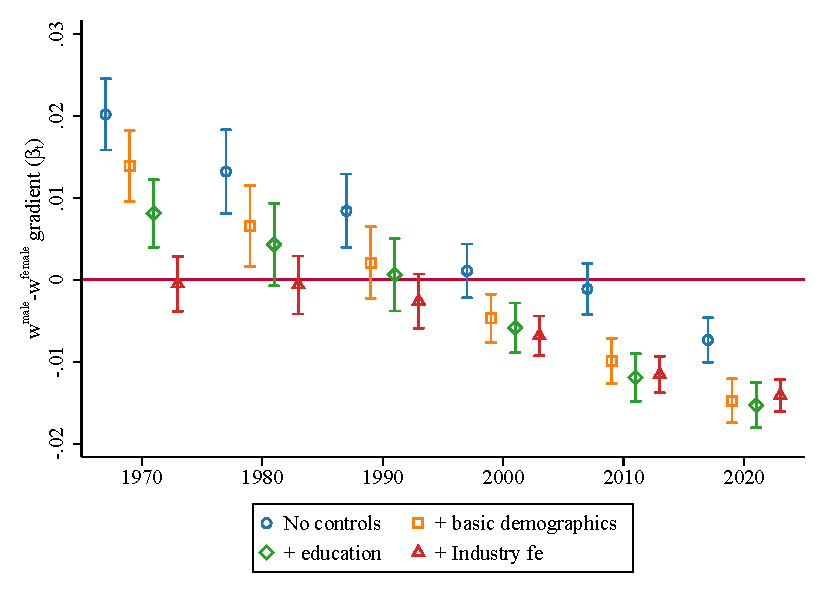
\includegraphics[width=.6\textwidth]{../2_analysis/output/figures/with_control_gradients_individual_l_czone_density_full_time}
\par \begin{minipage}[h]{\textwidth}{\tiny\textbf{Note:} figure restricts to CZ with more than 1 people per km$^2$. The regressions are done on data aggregated at the CZ level after residualizing individual-level characteristics. Bars show 95\% confidence intervals. Errors clustered at the CZ-level.}\end{minipage}
\end{figure}

	\beamerbutton{\hyperlink{slide:residual}{How do I control for individual characteristics?}}
\end{frame}

\begin{frame}{Adding czone-level variables}
	\label{slide:cz_controls}
	\textbf{\alert{Regression specification:}} $w^{men}_{rt}-w^{women}_{rt}=\alpha_{rt}+\beta_{t}\ln(density)_t+X_{rt}\gamma_t$
	\begin{figure}[!h]
\centering
\caption{Coefficient on population density $ \beta_t $ controlling for worker characteristics}
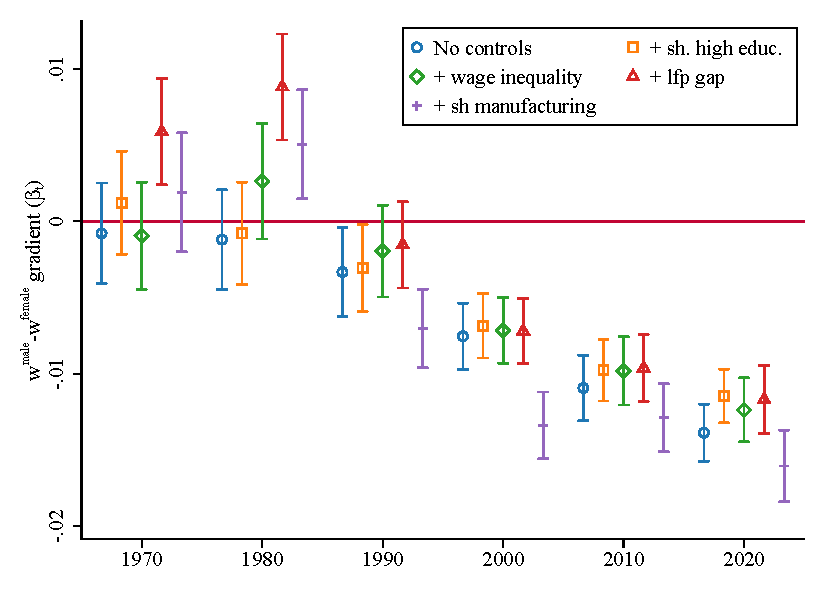
\includegraphics[width=.6\textwidth]{../2_analysis/output/figures/with_control_gradients_czone_l_czone_density_full_time}
\par \begin{minipage}[h]{\textwidth}{\tiny\textbf{Note:} figure restricts to CZ with more than 1 people per km$^2$. Regression includes census division $\times $ year fixed-effects. Additional controls include number of children, marital status and being a female head of household. The regressions are done on data aggregated at the CZ level. Bars show 95\% robust confidence intervals. Standard errors clustered at the CZ level. Figure generated on 19 Oct 2020 at 19:41:29. Figure generated using the dofile 2\_analysis/code\_files/write\_regression\_coefplots.do.}\end{minipage}
\end{figure}

	\beamerbutton{\hyperlink{slide:residual}{How do I control for individual characteristics?}}
\end{frame}